
\begin{figure}[htbp]
\centering
\vspace{-2mm}
 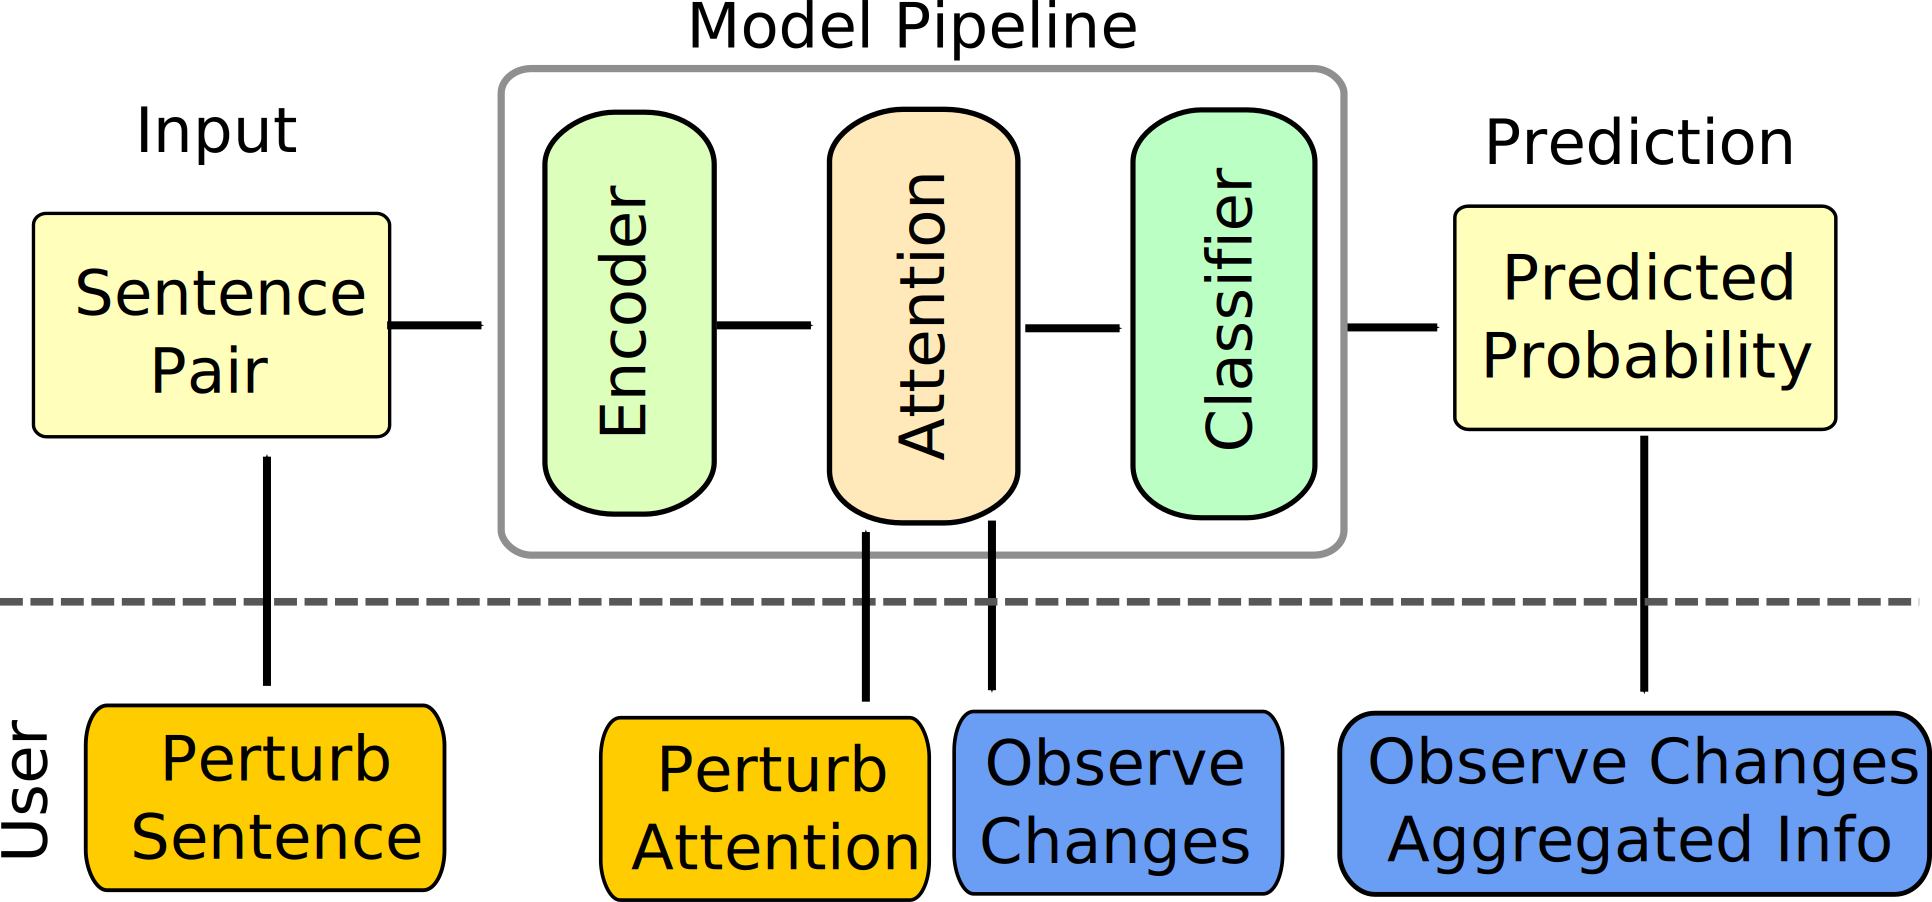
\includegraphics[width=1.0\linewidth]{pipeline}
 \caption{
 Perturbation-driven exploration of the end-to-end models that follows the encoder, attention, and classifier structure. The user can generate small perturbation of the input (i.e., replacing synonyms, paraphrasing)
 }
\label{fig:modelPipeline}
\end{figure}

\section{Visualization System}
As illustrated in Figure~\ref{fig:modelPipeline}, many recent end-to-end NLP model follows a similar encode, attent, and classify structure, in which the attention stage provide a window for peeking into the model decision making process. However, the static attention alone likely does not tell the whole story, instead we can learn more about the model by examining the dynamic between the input, the attention, and the output. To explore the relationship between different components of the pipeline, the proposed system utilizes a perturbation-driven exploration strategy, where the  user can manually or automatically generate small changes in the input sentence and then view the aggregated prediction information. Beside the perturbation of the input, the system also allows interactive modification of the attention values, where the prediction will instantaneously updated to reflect the changes. 
%

\subsection{Input Sentences Perturbation}
\label{sec:perturb}
Due to the discrete nature of the natural language, applying perturbation to sentence for sensitivity analysis can be particularly challenging compared to other problem domain, as small changes in words can leading to drastic different in the semantics of the sentences.
To reduce the potential semantic deviation, we first devise a simple perturbation method by replacing \emph{nouns} and \emph{verbs} by their synonyms in the wordNet~\cite{Miller1995}. However, the limitation is apparent, as synonyms replacement does not guarantee the meaning of the sentence remain the same. And the wordNet also has a rather inclusive definition for synonyms, where many infrequent/obscure usages exists, which leads to less meaningful perturbed sentence. However, this method requires minimal computation and easy to code and understand. 

\begin{figure}[htbp]
\centering
\vspace{-2mm}
 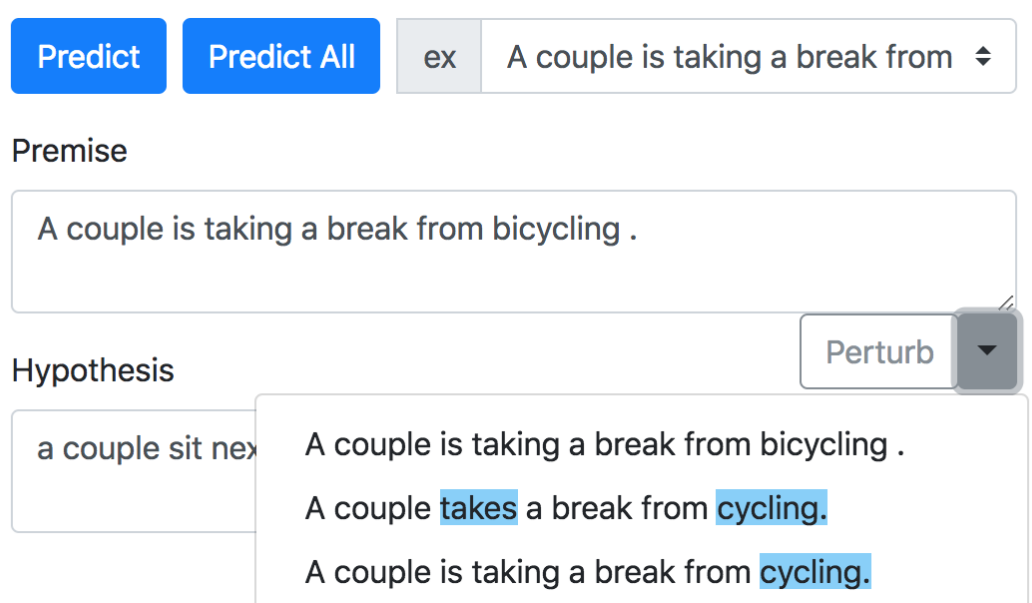
\includegraphics[width=1.0\linewidth]{sentence}
 \caption{
The interface for showing input sentences. The user can manually alter the words or apply automatic perturbation/paraphrasing of the inputs. In the \emph{perturbed} dropdown menu, the blue words are the only not exist in the original sentence.
 }
\label{fig:sentence}
\end{figure}

To improve the perturbation quality, we also adopted a translation based paraphrasing technique that is similar to the method discussed in \cite{mallinson2017paraphrasing}. Here, we translate the original English sentence into several other languages are then translate back into the English. Provided the translation produce correct result, we essential obtain paraphrasing of the original sentences (see Figure~\ref{fig:sentence}, where the drop-down menu shows the paraphrased/perturbed sentence).


\begin{figure*}[t]
\centering
\vspace{-2mm}
 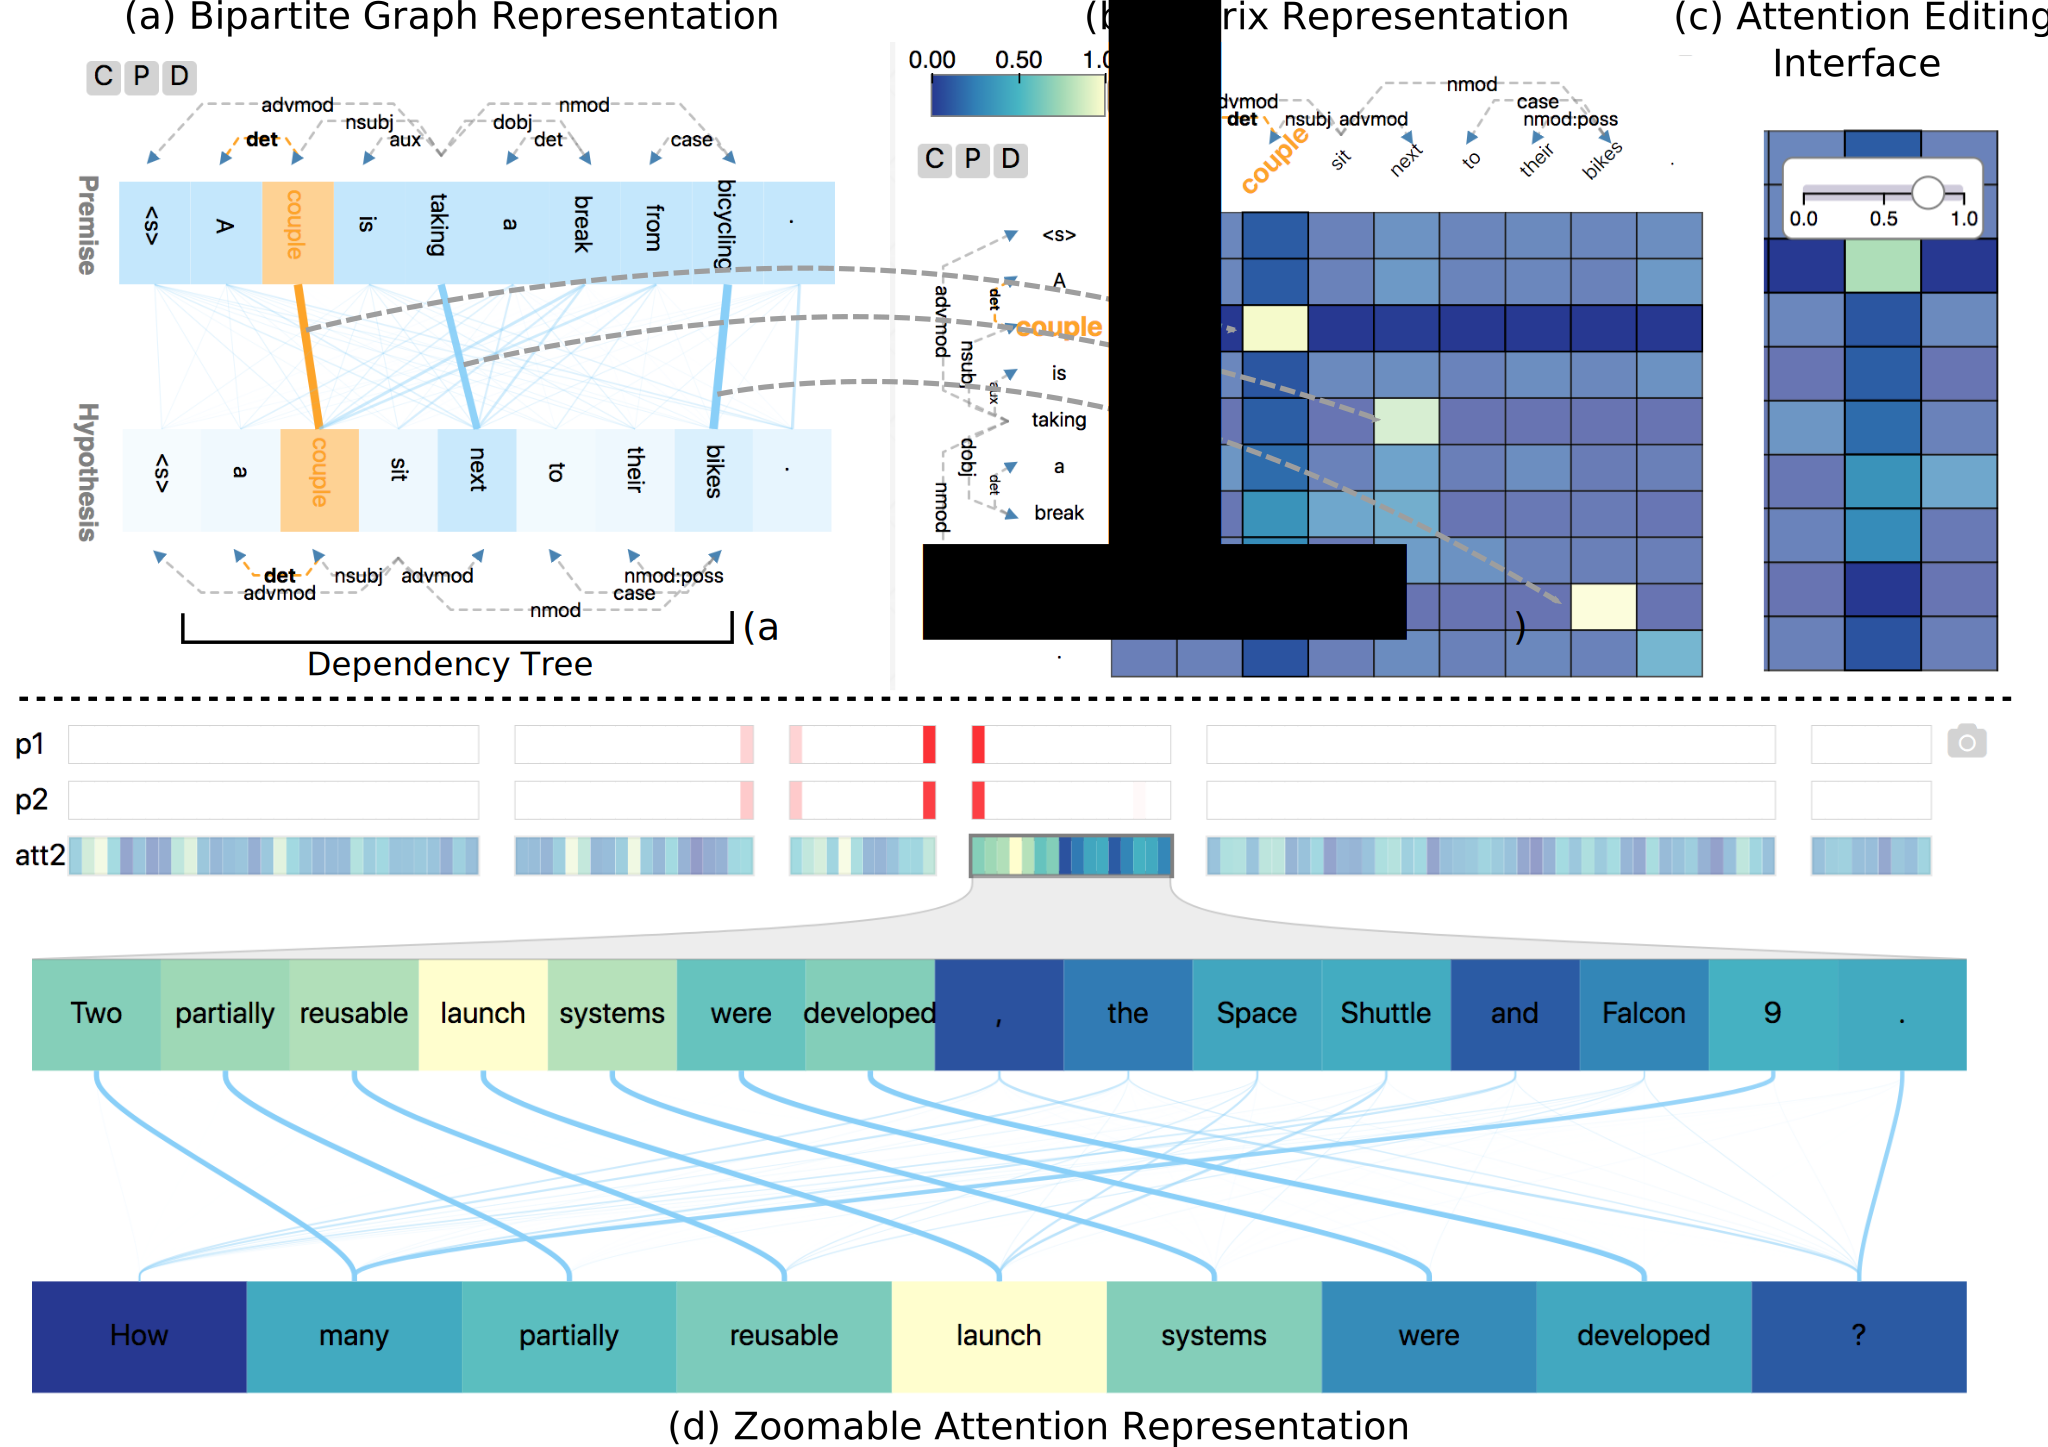
\includegraphics[width=1.0\linewidth]{attentionPanels}
  \vspace{-6mm}
 \caption{
Attention visualization. In the graph attention view (a), a bipartite graph encoding is adopted, in which the edge thickness corresponds to the attention value. In the matrix attention view (b), the entries of $i^{th}$ row represent the probabilities of words in hypotheses align to the $i^{th}$ word in the premise.
The user can alter the attention values via the pop-up interface illustrated in (c).
We overlay the dependency tree ($a_1$) grammar structure to highlight important words and allow simplification of complex sentence based on the dependency tree.
%
For highly asymmetric attention relationship, we utilized a zoomable hierarchical visual representation (d).
}
\label{fig:attentionVis}
\end{figure*}

\subsection{Attention Visualization}
The system consistence several visualization components that can be combine to generate an functional interactive system. Here we will focus on the attention visualization components. 
As illustrated in Figure~\ref{fig:attentionVis}(a)(b), the most widely adopted technique to bipartie graph (a), as well as the heatmap attention matrix representation (b). 
%
In the graph attention view (Fig.~\ref{fig:attentionVis}(a)), a bipartite graph encoding is adopted, in which the edge thickness corresponds to the attention value. The color of the rectangle text block encodes the sum of all edge values connected to it (darker shade of blues correspond to higher values).
%%%%%%%%
The graph view is suitable for highlighting the most dominant alignments. However, the edges may become cluttered if multiple attention values are high. The matrix attention view (Fig.~\ref{fig:attentionVis}(b)) resolve these issues, despite being more verbose and less efficient in highlighting the dominant alignments. 
%Together, the graph and matrix views complement each other and provide the same information from different perspectives. As illustrated by the pink arrowed lines, we can see how the same attention value is visualized in both the graph and the matrix view.
To help the user recognize the correspondence during the exploration, we enable the linkage between highlighted actions in both views (see Fig.~\ref{fig:attentionVis}(a)(b), the attention of the two ``couple'' is highlighted).
%
To address the challenge of visualizing long sentence, we incorporated the grammar structure.
One augmentation 

However, when the one of the text sequence become signification 





\subsection{Prediction Summarization}


\subsection{Implementation}
The initial setup cost and learning curve of the tool are often the barriers for user adaptation. To address these challenge, we design the visualization system as a Python library with modularity and easy accessibility in mind.
Instead of using the visualization system as a monolithic standalone application, just like a plotting library (i.e., matplotlib), the different pieces of the visualization (i.e., matrix based attention encoding) can be accessed individually.
% 
Yet, the components can also be combined in any configuration desired by users via a simple API to better fit into one's workflow.
More importantly, the library-based design allows easy integration with the existing model implemented in Python.
%
To create a visualization, users only need to import the library, create an instance of the visualization object, and specify a set of callback functions, such as generating a prediction, accessing attention, to link the visualization to their NLP models. The the code required to create an interactive exploration environment for machine comprehension model is illustrated bellow.

\begin{lstlisting}[language=Python, caption=Code for setting up the visualization system shown in the paper.]
from visPackage import MCModule
from bidaf_src import bidafModelInterface
from NLPutility import translationPerturbation

#initialize machine comprehension model
model = bidafModelInterface(
    wordDict="data/bidaf/squad.word.dict",
    wordVec="data/bidaf/glove.hdf5",
    model="data/bidaf/bidaf.ema")

gen = translationPerturbation()

# visualization components
visLayout = {
  "column":[{"row": ["Paragraph", 
                     "AttentionSubMatrix"]},
            {"row": ["AttentionAsymmetric"]}]
  }

#setup interface
modelVis = MCModule(visLayout)

modelVis.setPredictionHook(model.predict)
modelVis.setAttentionHook(model.attention)
modelVis.setSentenceHook(gen.perturbSentence)

#open browser for the web-based visualization
modelVis.show()
\end{lstlisting}



